\documentclass[12px]{article}
% \usepackage{amsmath}
\usepackage[fleqn]{amsmath}
\usepackage{amssymb}
\usepackage{caption}
\usepackage{subcaption}
\usepackage{graphicx}
\usepackage{cancel}
\usepackage{titling}

\usepackage{hyperref}
\hypersetup{
colorlinks=true,
linkcolor=blue,
filecolor=magenta,
    urlcolor=blue,
}
\urlstyle{same}

\graphicspath{ {./images/} }

\newcommand{\R}{\mathbb{R}}

\begin{document}

    \title{ECH 267 Nonlinear Control Theory \\ Homework \#1  }

    \author{Jonathan Dorsey: Department of Mechanical \& Aerospace Engineering}


    \maketitle


    \begin{center}
        \section*{Github Repo Hosted at: }
        \url{https://github.com/JonnyD1117/ECH-267-Adv.-Proc.-Control}
    \end{center}




\section*{Problem \#1}
Consider a single-input-single-output system described by the nth-order differential equation.

\[ y^{(n)} = g_{1} \left(t, y, \dot{y}, ... ,y^{(n-1), u}  \right) + g_{2} \left( t, y, \dot{y}, ... ,y^{(n-2)}\right)\dot{u}   \]

where $g_{2}$ is a differentialable function of its arguments. With $u$ as input and $y$ as output, find the state-space model. Hint: $x_{n} = y^{(n-1)} - g_{2} \left( t, y, \dot{y}, ..., y^{n-2}\right)$ \\

\textbf{Solution:} The first step is to define the state variables and then to determine the state-space model by constructing the $n-th$ first-order ODE system as follows...\\

State Definitions:
\begin{flalign*}
    & x_{1} = y \\
    & x_{2} = \dot{y} \\
    & \vdots \\
    & x_{n-2} = y^{n-3} \\
    & x_{n-1} = y^{n-2}\\
    & x_{n} = y^{n-1} - g_{2} \left( t, y, \dot{y}, ..., y^{n-2}\right) \\
\end{flalign*}

State Derivative Definitions:
\begin{flalign*}
    & \dot{x_{1}} = x_{2} \\
    & \dot{x_{2}} = x_{3} \\
    & \vdots \\
    & \dot{x}_{n-1} = y^{n-1}\\
    & \dot{x}_{n} = y^{n} - g_{2} \left( t, y, \dot{y}, \cdots , y^{n-2}\right)\dot{u} - \left( \frac{\partial g_2}{\partial t} + \frac{\partial g_2}{\partial x_1} \cdot \frac{\partial x_1}{\partial t} + \cdots \frac{\partial g_2}{\partial x_{n-1}} \cdot \frac{\partial x_n}{\partial t} \right) u\\
\end{flalign*}

\noindent Where the final derivative $\dot{x}_{n}$ is found by using the chain rule on the expression for $x_{n}$, since $g_2$ is a differentiable function. To accomplish this, we can expand the derivative using the product rule of differentiation, to obtain the final form of $\dot{x}_{n}$.

\section*{Problem \#2}

Given the block diagram of the system, we can define the following expressions and substitute them together with the standard linear state-space model to arrive at the new closed loop state-space model, as a function of $\psi(t, y)$.


    $$\dot{x} = A x + Bu $$
    $$y = Cx + Du $$

\noindent From the block diagram, it is obvious that the control input is defined as follows.
$$ u = r - \psi(t,y) $$

\noindent By substituting this expression for the control input, we can derive the final state-space form of...

$$  \dot{x} = Ax + B\left( r - \psi(t,y) \right) $$
$$ y = Cx + D(r - \psi(t,y)) $$

\section*{Problem \#3}

Consider the nonlinear system
$$
\begin{array}{l}
\dot{x}_{1}=h(t) x_{2}-g(t) x_{1}^{3} \\
\dot{x}_{2}=-h(t) x_{1}-g(t) x_{2}^{3}
\end{array}
$$
where $h(t)$ and $g(t)$ are bounded continuously differentiable functions, with $0<g_{0} \leq g(t)$.


\begin{itemize}
  \item (a) Is the equilibrium $x=0$ uniformly asymptotically stable? Is it globally uniformly asymptotically stable?
  \item (b) Is it (globally/locally) exponentially stable?
\end{itemize}



\subsection*{Solution Problem 3}

To investigate the stability properties of this system, we can use Lyapunov Stability Theory. We can construct a Lyapunov Candidate function $V(x)$ such that.

$$
V(x) = \frac{1}{2} x_1^2 + \frac{1}{2} x_2^2
$$

\noindent By taking the time derivate of $V$...

$$
\dot{V}(x) = x_1\dot{x_1} + x_2\dot{x_2}
$$

\noindent We can further expand this expression by substituting the state equations.

$$
\begin{aligned}
\dot{V}(x) & = x_1\left( h(t) x_2 -g(t) x_1^3 \right) + x_2\left(-h(t) x_1 -g(t) x_2^3 \right) \\
& = x_1x_2h(t) -x_1x_2h(t) - x_1^4g(t) -x_2^4g(t)
\end{aligned}
$$

\noindent After canceling terms, we get that the Lyanpunov function for this problem is...
$$
\dot{V}(x) = - x_1^4g(t) -x_2^4g(t)
$$

\noindent According to Theorem 4.8 (Khalil), we state that a equilibrium point is \underline{uniformly stable}, if we can show that



$$
  W_1(x)\leq V(t,x) \leq W_2(x) \\
$$
$$
\frac{\partial V}{\partial t} + \frac{\partial V}{\partial x}f(t,x) \leq 0
$$

\noindent $\forall t \geq t_0$ and $\forall x \in D$\\

\noindent Where the function $W_1$ and $W_2$ are positive definite functions. The reasoning is that for $V$ to obey this property $V$ must itself be positive definite, while for time derivative of $V$ must be at negative semi-definite. Additionally, inorder for this theorem to hold, it must be shown that these properties are independent of time. \\

\noindent However, in order to show that the system is \underline{Uniformly Asymptotically Stable}, we need a stronger condition. This condition is...

$$
\frac{\partial V}{\partial t} + \frac{\partial V}{\partial x}f(t,x) \leq - W_3(x)
$$

\noindent Where $W_3$ is also a positive definite function. This condition implies that there must exist a bound on the values of $\dot{V}(t,x)$ such that $\dot{V}$ is \textbf{always} be strictly less than zero. Using this information we can show whether or not the system is uniformly asymptotically stable.


\subsubsection*{Part A}
It is trivial to show that the candidate function $V(x)$ is positive definite $\forall x \in \R^2$, since by its constructed of even powers and since each term is negated the function must be $V(x) > 0 \quad \forall x \in \R^2 - \{0\}$ and $V(0)=0$. However, inorder to demonstrate that the theorem above holds, we mut show that the function $\dot{V}(x)$ is strictly negative definite. \\

\noindent Given the Lyapunov function...

$$
\dot{V}(x) = - x_1^4g(t) -x_2^4g(t)
$$

\noindent In order to ensure that this function stays negative definite over the entire domain $\forall x \in \R^2$, it must be shown that $g(t)$ term does not impact the negative definite-ness of $\dot{V}$. Since we are given that...

$$ 0<g_{0} \leq g(t)$$

\noindent We know that the value of $g(t)$ will always remain greater than zero, by definition. This tells us that $\dot{V}(x)>0$, $\forall x \in \R^2 $ and that $\dot{V}(0) = 0$ at the equilibrium point of the system. Since this function is negative definite, it is possible to find a positive definite function that satisfies the relationship for $W_3$ presented above. \\

\noindent Therefore according to \textbf{Theorem 4.8} and \textbf{Theorem 4.9} (Khalil), we have shown that there exists a positive definite function $V(x)$which can be upper and lower bounded by other PD functions, and that there exists a function $\dot{V}$ that is strictly negative definite, BOTH of which are independent of the initial time of the system $t_0$. Therefore we can conclude that the system is \underline{\textbf{Uniformly Asymptotically Stable}}! \\

\noindent Additionally, since we can find a function $W_1$ that is radially unbounded (\textbf{Theorem 4.9}), and since all of the former properties hold for the entire domain $\forall x \in \
R^2$ and not just a subset $D \subset \R^2$, we can conclude that the system is also \underline{\textbf{Uniformly Globally Asymptotically Stable}}.





\subsubsection*{Part B}

In order to determine whether the system is (globally/locally) exponentially stable, we must establish by \textbf{Theorem 4.10} (Khalil), that there exists constants $k_1$, $k_2$, $k_3$, and $a$ such that ...

$$
k_{1}\|x\|^{a} \leq V(t, x) \leq k_{2}\|x\|^{a}
$$
$$
\frac{\partial V}{\partial t}+\frac{\partial V}{\partial x} f(t, x) \leq-k_{3}\|x\|^{a}
$$

\noindent In order for to evaluate this, we only need to determine whether such constants exist. We can start by rewriting our candidate function in terms of its norm.

$$
V(x) = \frac{1}{2} \left\Vert x \right\Vert_2^2
$$

\noindent It is relatively straightforward to demonstrate that we can satisfy the first condition, with $k_1 = .25$, $k_2 = 1$, $a=2$.

$$
\frac{1}{2} \left\Vert x \right\Vert_2^2 \leq V(x) \leq \left\Vert x \right\Vert_2^2
$$


\noindent The final task to determine whether there is a constant $k_3$ such that ...

$$
- x_1^4g(t) -x_2^4g(t) \leq -k_3 \left\Vert x \right\Vert_2^2
$$


\noindent While it is possible that I am not seeing the pattern or simplifying the form the correct way, I cannot find a constant $k_3$ for this specific Lyapunov function that demonstrates that the system is exponentially stable, therefore I think that the system is \textbf{NOT} \underline{\textbf{Exponentially Stable}}. \\

\noindent My reasoning for this decision that for the Lyapunov function that I constructed to solve this problem, it is very hard to relate the 2-norm of the $x$ to $- x_1^4g(t) -x_2^4g(t)$. This makes it hard to reduce the problem down to its core. Since as far as I can tell, this expression does not simplify (such defining a ball of a certain radius and using that to get the form of eqach side of the inequality to be more or less comparable), then it appears to me that the there are obvious values of $\forall x \in \R^2$ that would require a different $k_3$ to satisfy the inequality. In particular, the when the value of $x_1<1, x_2 <1$, would require a significantly different $k_3$ than when $x_1 >1, x_2 >1$.

\section*{Problem \#4}


Consider the nonlinear system:
$$
\dot{x}=f(x), \quad x(0)=x_{0}
$$
where $f(0)=0 .$ Assuming that $f: D \rightarrow \mathbb{R}^{n}$ is Lipschitz on its domain and let solutions of the system be bounded by:
$$
\|x(t)\| \leq \beta(\|x(0)\|, t)
$$
for $\|x(0)\|<c$ for some $c>0$ where $\beta \in \mathcal{K} \mathcal{L} .$ Show that the origin is asymptotically stable in the sense of the classical asymptotic stability $(\epsilon-\delta)$ definition.



\begin{center}
  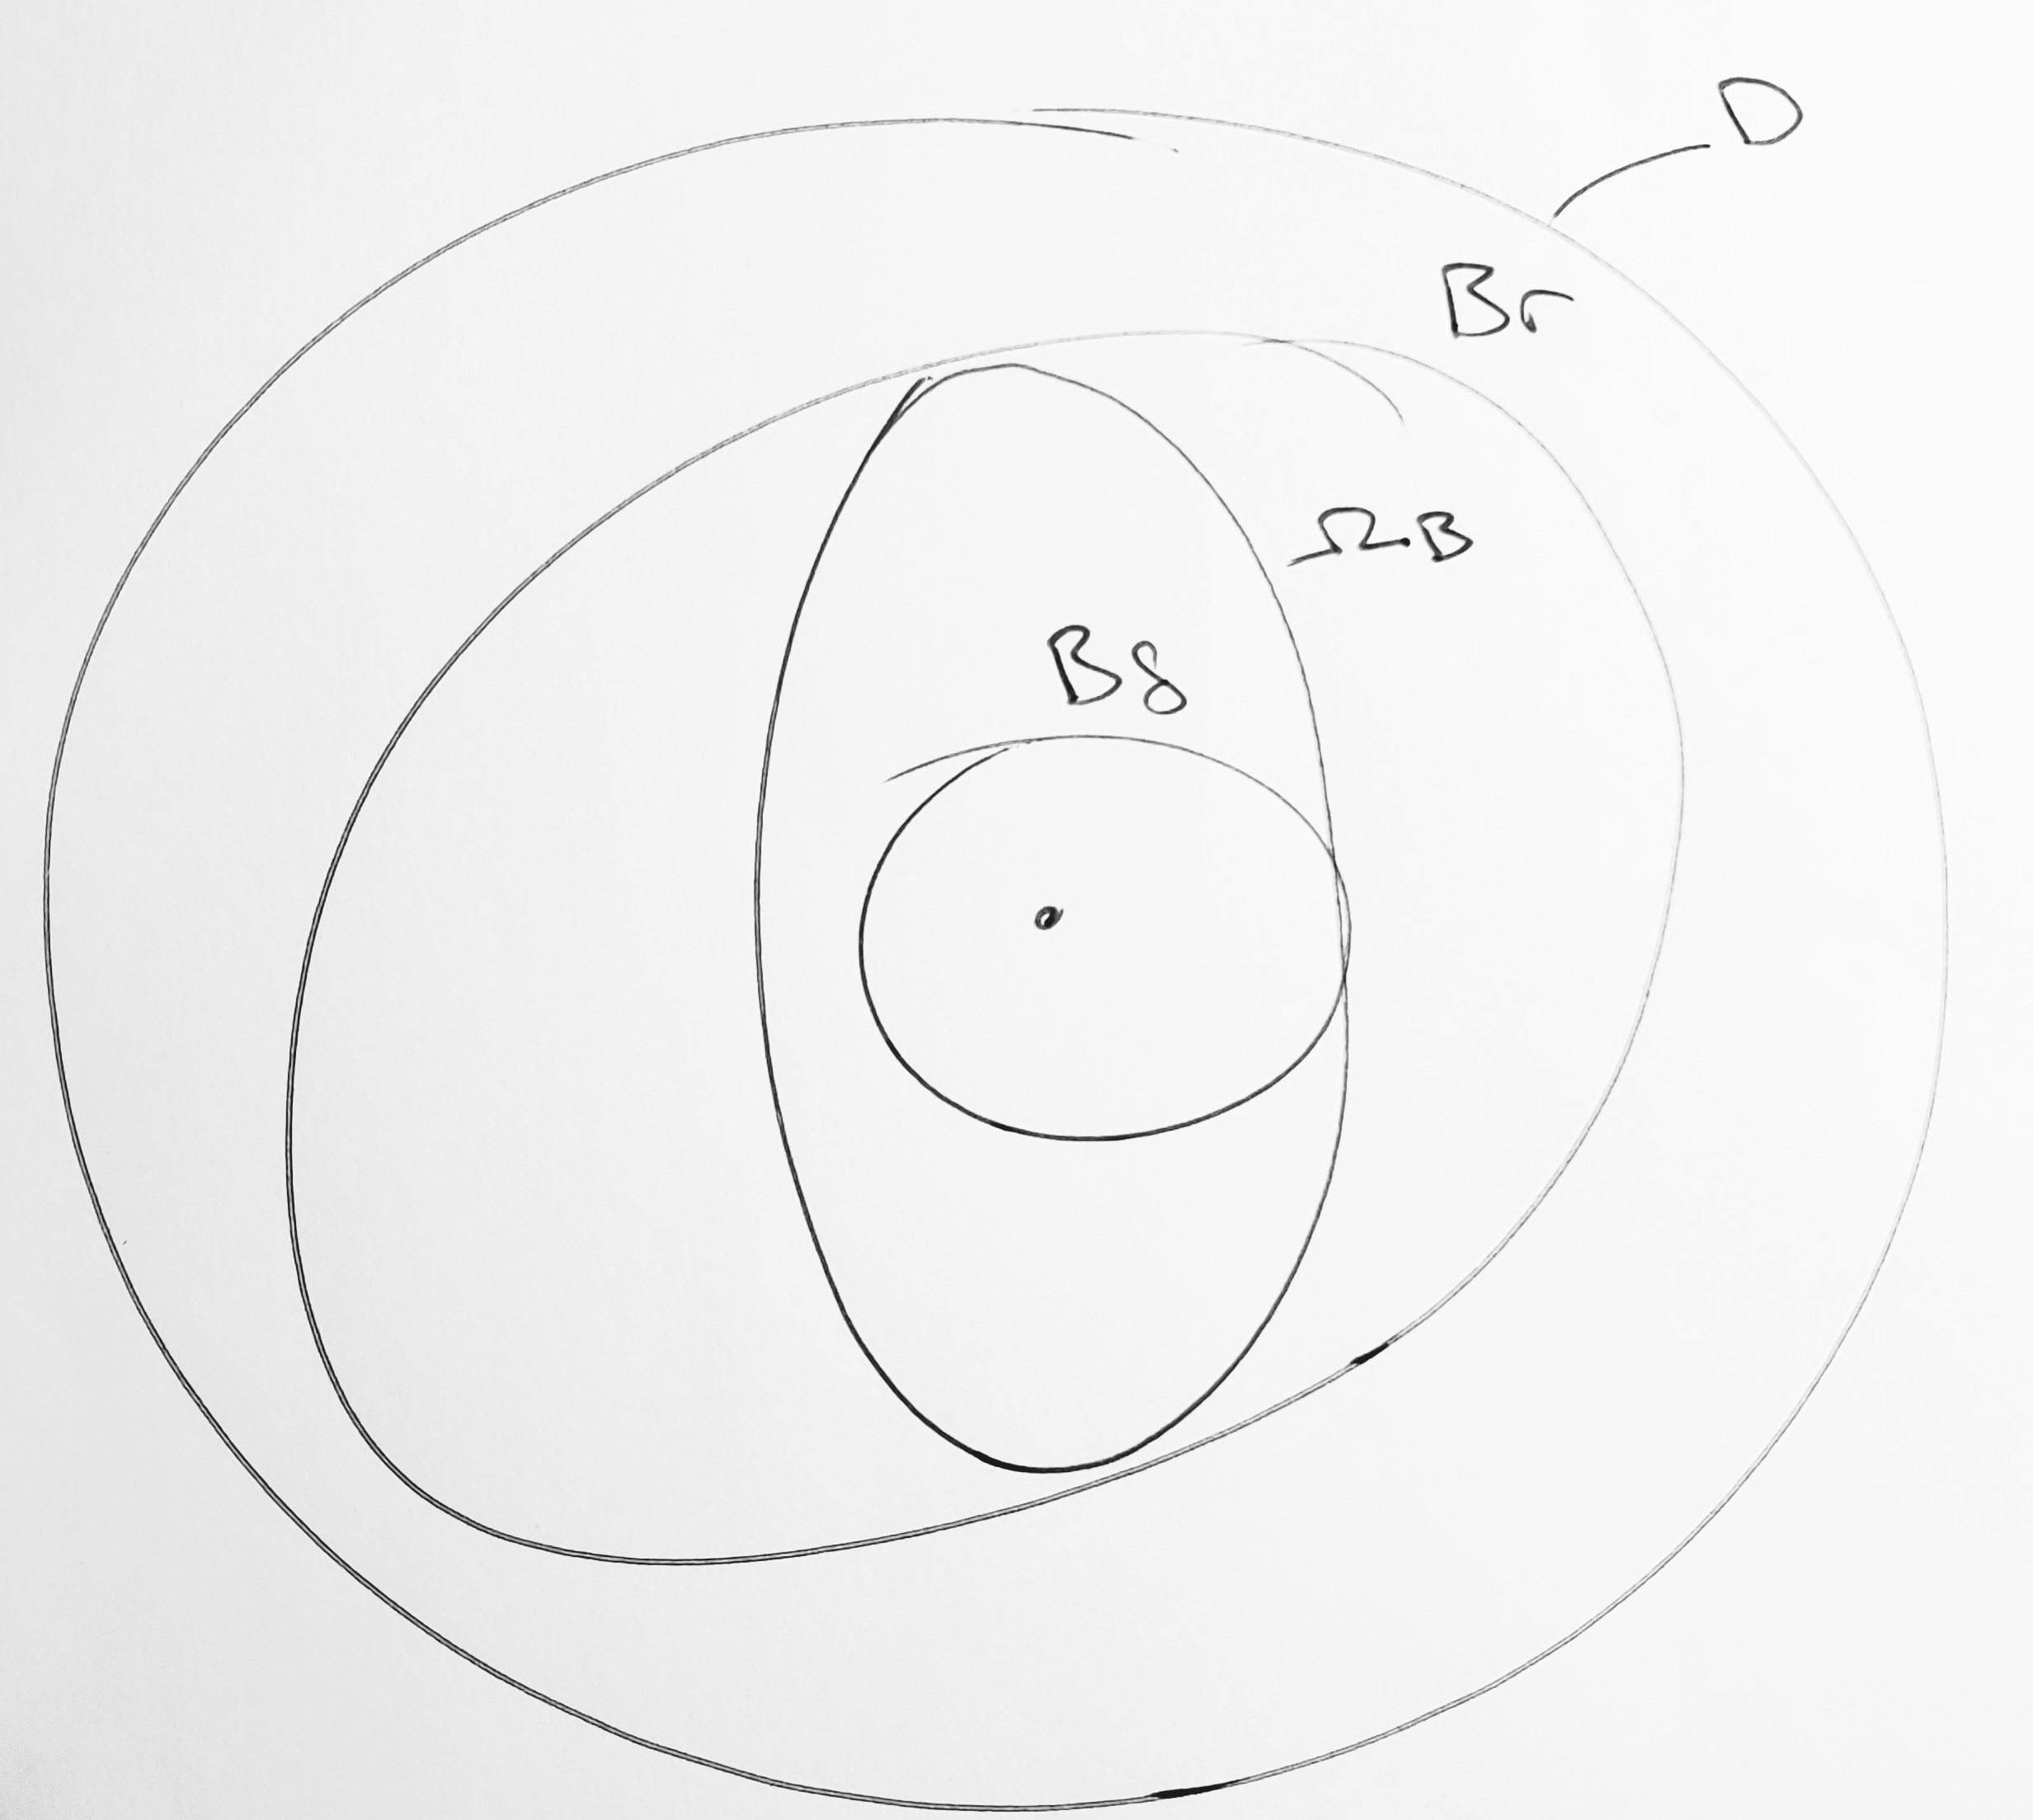
\includegraphics[scale=0.1]{proof}
\end{center}

\noindent In order to demonstrate that the system (as defined using Comparison functions) is asymptotically stable, we need to demonstrate the $\epsilon - \delta$ proof of asymptotic stability and relate that to the usage of comparison functions to show the equivalence between the two. \\

\noindent For $\epsilon >0$ such that $r \in (0, \epsilon]$

$$
B_r = \{ x\in \R^n | \left\Vert x \right\Vert < r\} \subset D
$$

\noindent Then there is an $\alpha = min_{\left\Vert x \right\Vert = r} V(x)$, non-negative $\alpha >0$, such that $\beta \in (0, \alpha)$ we can define a positive invariant set $\Omega_B$ such that


$$
\Omega_B = \{ x \in B_r | V(x) \leq \beta\}
$$

\noindent Note that since, $\Omega_B$ is an invariant set, it has the property that any trajectory starting in it $x(t_0)$ remains in it such that $\left\Vert x(t) \right\Vert \in \Omega_B$. Due to this property we know that there must exist a function which is strictly decreasing such that ...


$$
V(x(t)) \leq V(x(t_0)) \leq \beta \quad \quad \forall t \leq t_0
$$

\noindent In order for this to be true

$$
\dot{V}(x) \leq 0
$$

\noindent It should be noted that $\Omega_B$ is a compact set by construction since it is a subset of $B_r$. From this fact, and under the assumptions listed in the problem statement, we can say that $\dot{x} = f(x)$ has a unique solution $\forall t \geq t_0$ for $X(t_0) \in \Omega_B$.\\

\noindent If $V(x)$ is continuous and $V(0) = 0$, we can define a $\delta$ such that..

$$
\left\Vert x \right\Vert \leq \delta \Rightarrow V(x) < \beta
$$

\noindent Since we know that ball of radius $\delta$ infers a value of $V(x)$ inside of ball of radius $\beta$, we can show that...

$$
B_{\delta} \subset \Omega_B \subset B_r
$$

\noindent If we start a trajectory inside of the ball of radius $\delta$ we can show that

$$
x(t_0) \in B_{\delta} \Rightarrow x(t_0) \in \Omega_B \Rightarrow x(t) \in \Omega_B \Rightarrow x(t) \in B_r
$$

\noindent This means that given this setup, from a given $\delta$ there must exist a $\epsilon$ (recall: $B_r$ defines the $\epsilon$) such that we can state.

$$
\left\Vert x(t_0) \right\Vert < \delta \Rightarrow \left\Vert x(t) \right\Vert < r \leq \epsilon, \quad \quad \forall t \geq t_0
$$


\noindent If this is true such this means that the system is stable according to the $\epsilon-\delta$ definition. However, this does not show that system is \underline{attractive}. In order to show that we need to prove that...

$$
x(t) \rightarrow 0 \quad \text{ as } t \rightarrow \infty
$$


\noindent Since the function $V(x(t))$ is decreasing we can show that if ...

$$
V(x(t)) \rightarrow c \geq 0 \text{ as } t \rightarrow \infty
$$

\noindent It is sufficient to show that the function $V(x) \rightarrow 0 $ as $t \rightarrow \infty$.

\subsection*{Solution Problem 4}

With the structure of the main proof out of the way, we need to show how the \underline{comparison functions} can be linked to this definition for asymptotic stabiilty. We can show that we can define the functions $V(t,x)$ and $\dot{V}(t,x)$ in terms of the comparison function $\alpha_i \in K$ and $\beta_i \in KL$. From the definitions of the classes (K, KL) we can show that in order for the function $V$ to be positive definite it must be able to be upper and lower bounded by functions $\alpha_1(\cdot)$ and $\alpha_2(\cdot)$. \\

$$
\alpha_1(\left\Vert x \right\Vert) \leq V(t,x) \alpha_2(\left\Vert x \right\Vert)
$$

\noindent In addition to this, we must show that the function $\dot{V}(x)$ is negative definite, which can be stated as $\dot{V} \leq -\alpha_3(\cdot)$. We can observe that via Lemma 4.2, that by using properties of these functions we can rewrite

$$
V(t,x) \leq \sigma(V(t_0, x(t_0)), t- t_0), \quad \forall V(t_0, x(t_0)) \in [0,c]
$$

\noindent which can be written

$$
\left\Vert x \right\Vert \leq \beta(\left\Vert x(0)\right\Vert, t)
$$

Since it is possible to rewrite the original statement of asymptotic stability in terms of comparison functions, we can show the direct connection between the form of the problem given and the direct $\epsilon-\delta$ proof of asymptotic stability.

\section*{Problem \#5}

Given the following equation over $[0, \infty)$...

$$
\dot{x}(t) = [x(t)]^{\frac{1}{3}} \hspace{.3cm}, x(0) =0\\
$$

\noindent We can show that this problem has a \textbf{NOT unique} solution, via the ``Existance and Uniqueness Theorem''. \\

\noindent This theorem states that if the function and its derivative are continuous around the initial condition of the system that there exists a unique solution. \\

\noindent $\dot{x} = f(x)$ is a continuous function on the inteveral \textbf{not} including the origin, however, when taking the derivative of the function $f(x)$, we note that it is \textbf{not continuous} at $x=0$ where the function become undefined, according to the limit definition of a derivate. Since the limit approaching from the left and right do not agree, the derivative must not exist. Therefore we cannot say that the solution is unique due to the inclusion of the origin in the domain of the problem.

\section*{Problem \#6}

Consider the following nonlinear system:
$$
\begin{aligned}
\dot{x}_{1} &=f_{1}\left(x_{1}, x_{2}, x_{3}\right)+g_{1}\left(x_{1}\right) u \\
\dot{x}_{2} &=f_{2}\left(x_{1}, x_{2}, x_{3}\right) \\
\dot{x}_{3} &=f_{3}\left(x_{1}, x_{2}, x_{3}\right) \\
y &=h\left(x_{2}\right) \\
\end{aligned}
$$

\noindent Where $x_{1} \in \mathbb{R}$, $x_{2} \in \mathbb{R}$, $x_{3} \in \mathbb{R}$, $u \in \mathbb{R}$, $y \in \mathbb{R}$, $f_{1}(0,0,0)=f_{2}(0,0,0)=f_{3}(0,0,0)=0$ and $g_{1}(0) \neq 0$ .

\begin{itemize}
  \item (a) Determine the relative degree of the controlled output $y$ with respect to the manipulated input $u$.
  \item (b) Design an input/output feedback linearizing controller to stabilize the input/output dynamics.
  \item (c) State the conditions that ensure this controller enforces local asymptotically stability of the origin.
\end{itemize}


\subsection*{Solution Problem 6}


\subsection*{Part A}
To determine the \underline{relative degree} of the system we need to determine how many derivatives of the output $y$ must be taken inorder to see the effect of the input on the system. \\

\noindent This can be show by taking the generalized system form $ \dot{x} = f(x) + g(x)u $ and computing the Lie Derivaties.

$$
L_{g} L_{f}^{i-1} h(x)=0, \quad i=1,2, \ldots, \rho-1 ; \quad L_{g} L_{f}^{\rho-1} h(x) \neq 0
$$

\noindent This relation determines whether the derives of the output are independent of the input to the system. To begin this process for the given system, we need to take the Lie Derivative $L_g$ for $i = 1$ which gives ...

$$
L_gh(x) = \underbrace{\frac{\partial h}{\partial x_{1}} g_{1}(\cdot)}_0 + \underbrace{\frac{\partial h}{\partial x_{2}} g_{2}(\cdot)}_0 + \underbrace{\frac{\partial h}{\partial x_{3}} g_{3}(\cdot)}_0
$$

\noindent Therefore ...

$$
L_gh(x) = 0
$$

\noindent This indicates that the first derivative is \underline{independent} of the input. This means that we need to take the second derivate of the output and evaluate the system again, this time for $i = 2$.

$$
L_gL_fh(x) =
\frac{\partial}{\partial x}\left(\frac{\partial h}{\partial x} \cdot f\right) \cdot g
$$

\noindent In order to evluate this expression we need to compute $L_fh(x)$ and then compute the $L_g(L_fh(x))$.

$$
L_fh(x)= \frac{\partial h}{\partial x} f(x)=\frac{\partial h}{\partial x_{1}} f_{1}(\cdot)+\frac{\partial h}{\partial x_{2}} f_{2}(\cdot)+\frac{\partial h}{\partial x_{3}} f_{3}(\cdot)
$$


\noindent Since the function $h(x_2)$ is only dependent on $x_2$ derivatives of $h(x_2)$ with respect to $x_1$ and $x_2$ are zero.

$$
L_fh(x)= \underbrace{\frac{\partial h}{\partial x_{1}} f_{1}(\cdot)}_0 + \frac{\partial h}{\partial x_{2}} f_{2}(\cdot) + \underbrace{\frac{\partial h}{\partial x_{3}} f_{3}(\cdot)}_0
$$


\noindent Therefore

$$
L_fh(x)= \frac{\partial h}{\partial x_{2}} f_{2}(\cdot)
$$


\noindent To complete the process we need to take the following derivative

$$
L_gL_fh(x) = \frac{\partial}{\partial x} \left[ \frac{\partial}{\partial x_2}f_2(\cdot) \right] g(\cdot)
$$


\noindent We can expand this to...

$$
L_gL_fh(x) = \frac{\partial}{\partial x_1}(\frac{\partial}{\partial x_2}f_2(\cdot))\cdot g_1() + \underbrace{\frac{\partial}{\partial x_2}(\frac{\partial}{\partial x_2}f_2(\cdot))\cdot g_2()}_0 + \underbrace{\frac{\partial}{\partial x_3}(\frac{\partial}{\partial x_2}f_2(\cdot))\cdot g_3()}_0
$$


\noindent Since $g_1$ and $g_2$ are zero, the last two terms of the expression are cancelled out. This means that we can write.

$$
L_gL_fh(x) = \frac{\partial}{\partial x_1}(\frac{\partial}{\partial x_2}f_2(\cdot))\cdot g_1()
$$

\noindent Since this term does not reduce to zero we have determined that the system has a \underline{\textbf{Relative Degee}} = 2, since it took two time derivatives of the output to obtain an input/output relationship.


\subsection*{Part B}

We can directly find the input/output feedback linearizing controller, from the general equation, since our system is expressed in the general form $\dot{x} = f(x) + g(x)u$. The generalize linearizing input/output controller can be shown to be...


$$
u=\frac{1}{\operatorname{L_g} \operatorname{L_f} h(x)}\left[-L^{2}_f h(x) + v\right]
$$


\noindent Since we already have the expression for $L_gL_fh(x)$ from the previous problem, we only need to determine $L^2_fh(x)$ and the controller will be solved for.

$$
L_{f}\left(L_{f} h\right)=\frac{\partial}{\partial x}\left(L_{f} h\right)=\frac{\partial}{\partial x}\left(\left[\frac{\partial h(x)}{\partial x}\right] \cdot f(x)\right) \cdot f(x)
$$


$$
= \frac{\partial}{\partial x}\left(\left[\frac{\partial h(x_2)}{\partial x_2}\right] \cdot f_2(x)\right) \cdot f(x)
$$

\noindent By using prduct rules of calculus, this term expands to...
$$
L_{f}\left(L_{f} h\right) =  \frac{\partial}{\partial x_1} \left[ f_2() \right]\cdot f_1() +  \left[ \frac{\partial^2}{\partial x_2^2} (h(x_2))\cdot f_2() + \frac{\partial}{\partial x_2} (h(x_2))\cdot \frac{\partial}{\partial x_2}(f_2()) \right]  + \frac{\partial}{\partial x_3} \left[ f_2() \right] \cdot f_3()
$$

\noindent By substituting the derived expressions for $L_gL_fh(x)$ and $L^2_fh(x)$ into the feedback linearizing controller...
$$
u=\frac{1}{\operatorname{L_g} \operatorname{L_f} h(x)}\left[-L^{2}_f h(x) + v\right]
$$

We can design a controller that linearizes the nonlinear terms in the state equations and allows us to manipulate the system as if it was linear, and enabling the use of linear control techniques such as pole placement to control the system and keep it stable.

\subsection*{Part C}

Just linearizing the control input does not inherently make the system stable so in order to control the system and keep it stable we need to ensure the following ...

\begin{itemize}
  \item The system is in a form conducive to linerization $\dot{x} = f(x) + g(x)u$
  \item  The virtual input $v$ needs to enforce stable dynamics such that the closed loop system ($A - BK$) has stable poles in the \underline{left-half-plane} (aka Hurwitz)
  \item  The state space is controllable.
\end{itemize}


\section*{Problem \# 7}

\begin{itemize}
    \item (a): Determine the matrix M that transforms A into the appropriate modal form and write the system in model coordinates.
    \item (b): Classify the equilibrium (0, 0)
    \item (c): Generate the Phase Portrais of the system in both modal(z) and original(x) coordinates.

\end{itemize}

\subsection*{Part 7.A}
In order to determine the matrix M such that $\dot{z} = \left(M^{-1}AM \right)z$, for each of the matrices in the problem statement, such that the problem will be transformed into modal coordinates, we must first compute the eigenvalues and eigenvectors for each matrix. We can then compute the M matrix by concatenating the eigenvectors of the given matrix A, and finally we can find $M^{-1}$ by taking the matrix inverse of the M previously derived. By following these steps, we can transform A into its modal form. \\

To accomplish this, I utilized MATLAB to compute the eignvalues and eigenvectors, even though for these simple 2x2 matrices would be simple enough to compute by hand. However, these calculations would have been time consumming.

\subsubsection*{7.A.i}

Eigenvalue:
$$ \lambda = -1, -2 $$
Eigenvector:
$$M =
\begin{bmatrix}
    & .7071 & -.4472 \\
    & -.7071 & .8944
\end{bmatrix}
$$


\subsubsection*{7.A.ii}

Eigenvalue:
$$ \lambda = 1, 1 $$
Eigenvector:
$$M =
\begin{bmatrix}
    & -.7071 & -.7071 \\
    & .7071 & .7071
\end{bmatrix}
$$
\subsubsection*{7.A.iii}

Eigenvalue:
$$ \lambda = -1, 1 $$
Eigenvector:
$$M =
\begin{bmatrix}
    & 1 & -.4472 \\
    & 0 & .8944
\end{bmatrix}
$$
\subsubsection*{7.A.iv}

Eigenvalue:
$$ \lambda = \pm2j $$
Eigenvector:
$$M =
\begin{bmatrix}
    & .9129 & .9129 \\
    & -.1826 + .3651j & -.1826 - .3651j
\end{bmatrix}
$$
\subsubsection*{7.A.v}

Eigenvalue:
$$ \lambda = 1\pm1j $$
Eigenvector:
$$M =
\begin{bmatrix}
    & .4082+.4082j & .4082-.4082j \\
    & .8165 & .8165
\end{bmatrix}
$$

\subsection*{Part 7.B}
Classify the equilibrium at the origin for the different systems.
\subsubsection*{7.B.i}
The equilibirum at the origin for this system is a \underline{\textbf{Stable}}.

\subsubsection*{7.B.ii}
The equilibirum at the origin for this system is a \underline{\textbf{Unstable}}.

\subsubsection*{7.B.iii}
The equilibirum at the origin for this system is a \underline{\textbf{Saddle}}.

\subsubsection*{7.B.iv}
The equilibirum at the origin for this system is a \underline{\textbf{Unstable Focus}}.

\subsubsection*{7.B.v}
The equilibirum at the origin for this system is a \underline{\textbf{Unstable Focus}}.

\subsection*{Part 7.C}


\begin{figure}[h]
  \centering
  % 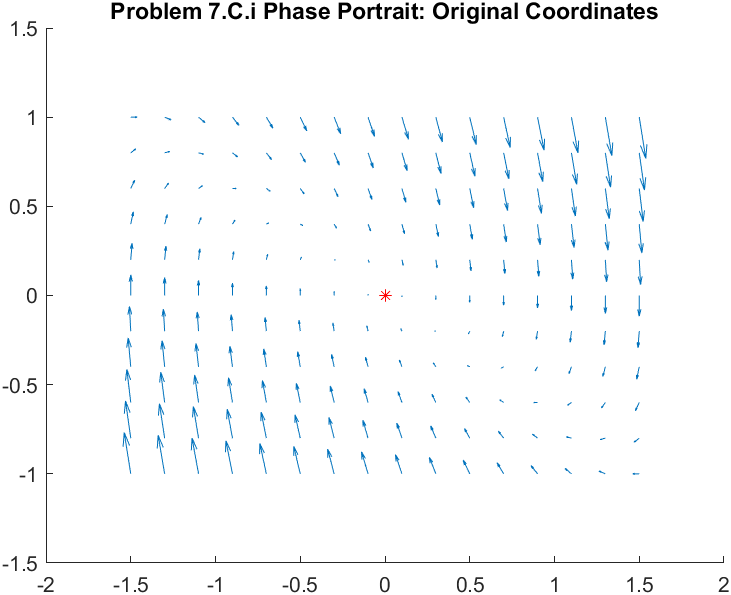
\includegraphics[width=\linewidth]{/prob7_img/7_C_i_Original}
  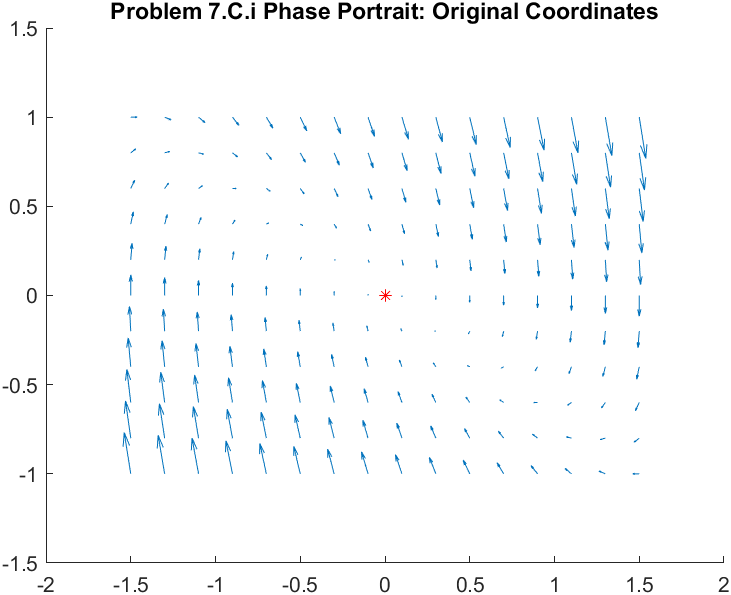
\includegraphics[width=\textwidth,height=.45\textheight,keepaspectratio]{/prob7_img/7_C_i_Original}
\end{figure}

\begin{figure}[h]
  \centering
  % 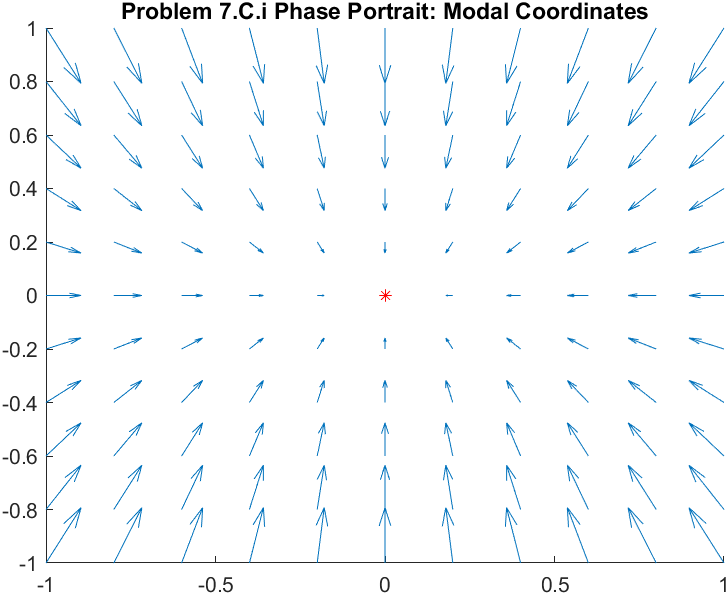
\includegraphics[width=\linewidth]{/prob7_img/7_C_i_modal}
  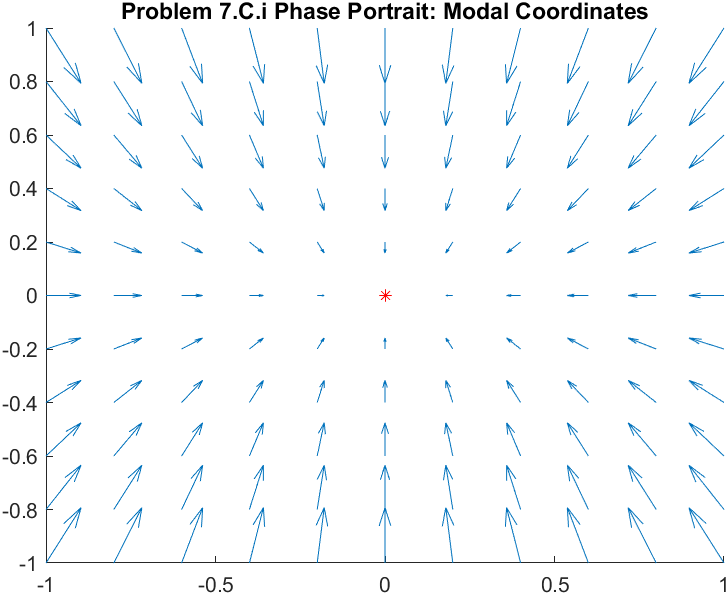
\includegraphics[width=\textwidth,height=.45\textheight,keepaspectratio]{/prob7_img/7_C_i_modal}

\end{figure}

\begin{figure}[h]
  \centering
  % 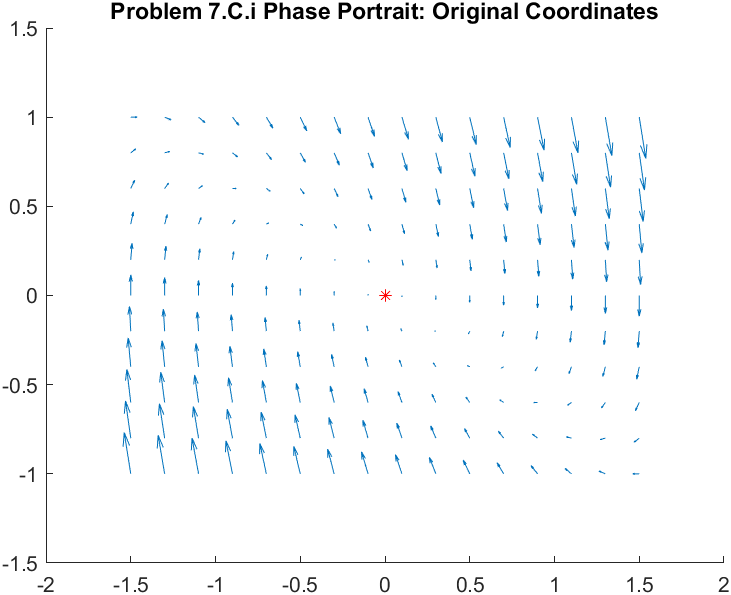
\includegraphics[width=\linewidth]{/prob7_img/7_C_i_Original}
  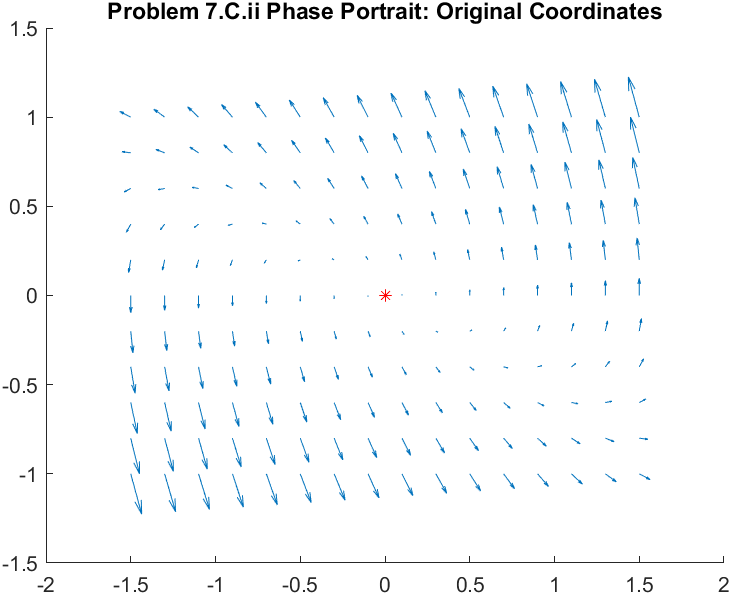
\includegraphics[width=\textwidth,height=.45\textheight,keepaspectratio]{/prob7_img/7_C_ii_Original}
\end{figure}

\begin{figure}[h]
  \centering
  % 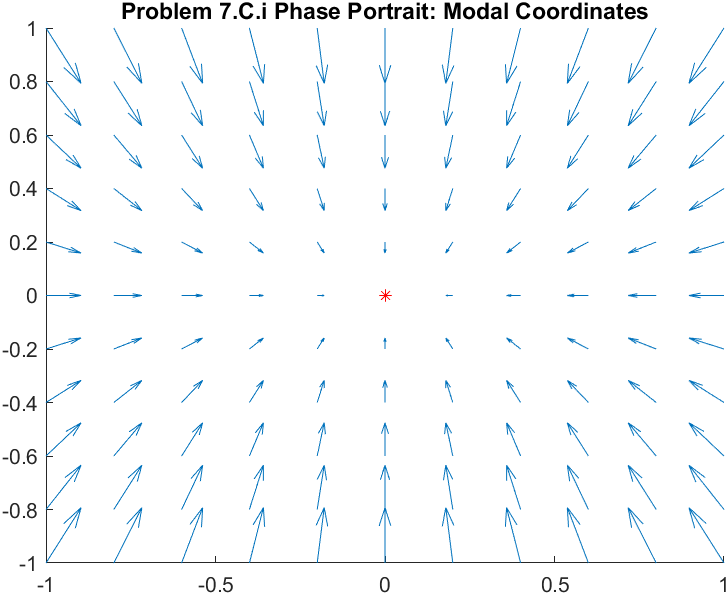
\includegraphics[width=\linewidth]{/prob7_img/7_C_i_modal}
  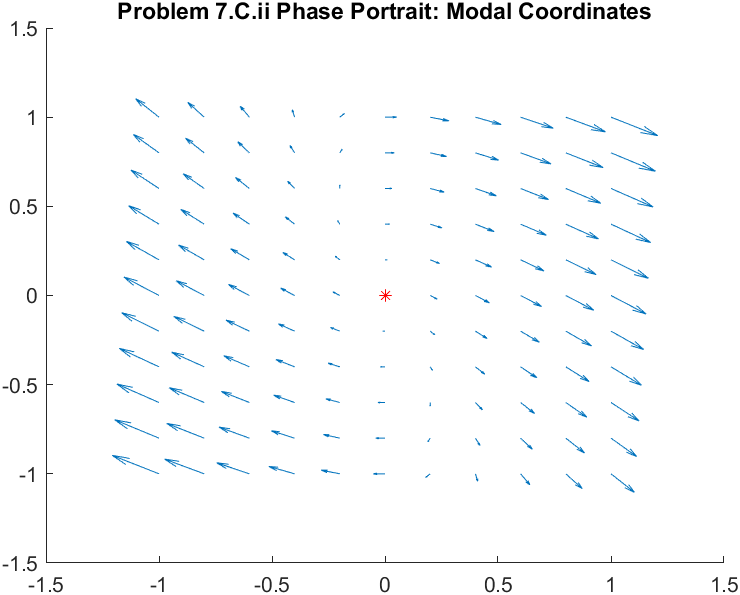
\includegraphics[width=\textwidth,height=.45\textheight,keepaspectratio]{/prob7_img/7_C_ii_modal}

\end{figure}

\begin{figure}[h]
  \centering
  % 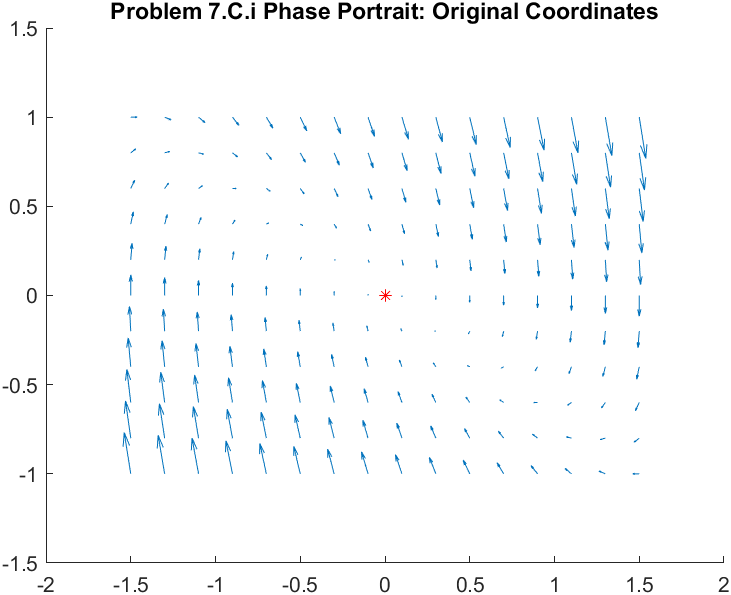
\includegraphics[width=\linewidth]{/prob7_img/7_C_i_Original}
  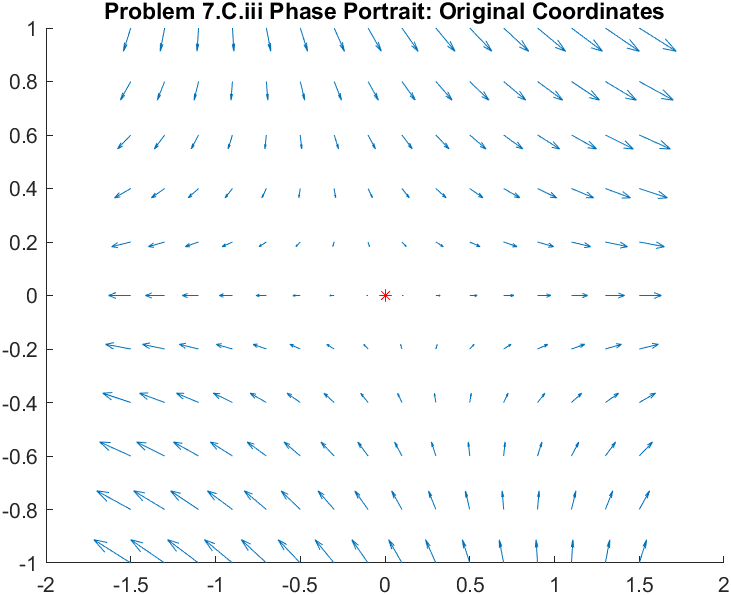
\includegraphics[width=\textwidth,height=.45\textheight,keepaspectratio]{/prob7_img/7_C_iii_Original}
\end{figure}

\begin{figure}[h]
  \centering
  % 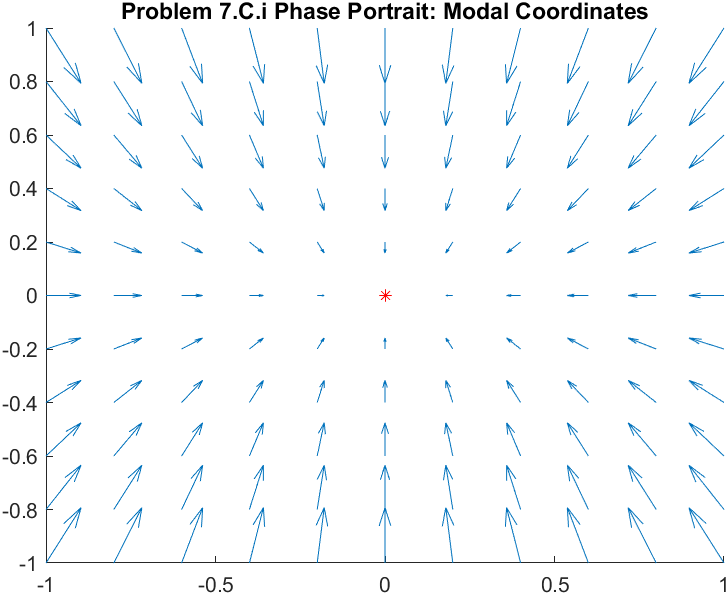
\includegraphics[width=\linewidth]{/prob7_img/7_C_i_modal}
  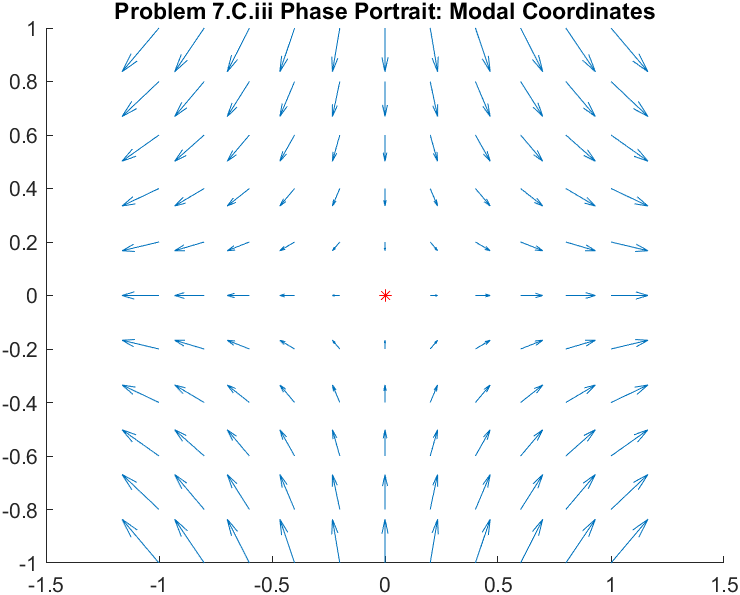
\includegraphics[width=\textwidth,height=.45\textheight,keepaspectratio]{/prob7_img/7_C_iii_modal}

\end{figure}

\begin{figure}[h]
  \centering
  % 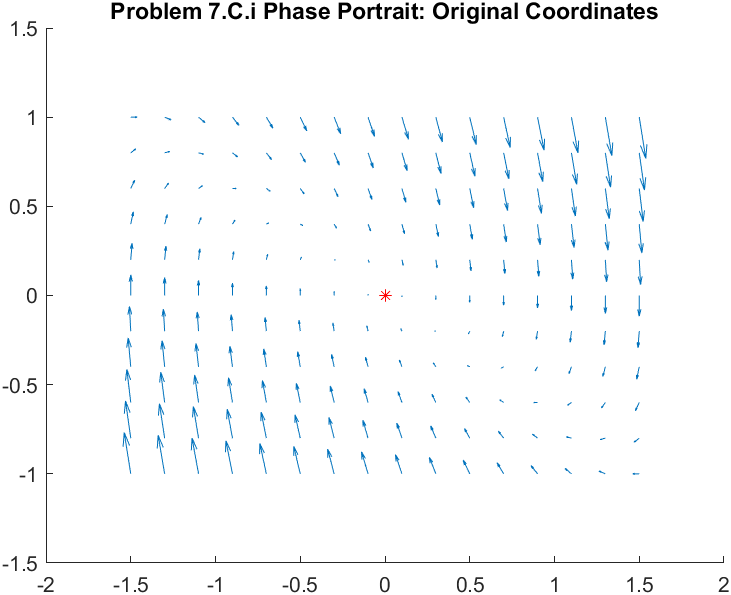
\includegraphics[width=\linewidth]{/prob7_img/7_C_i_Original}
  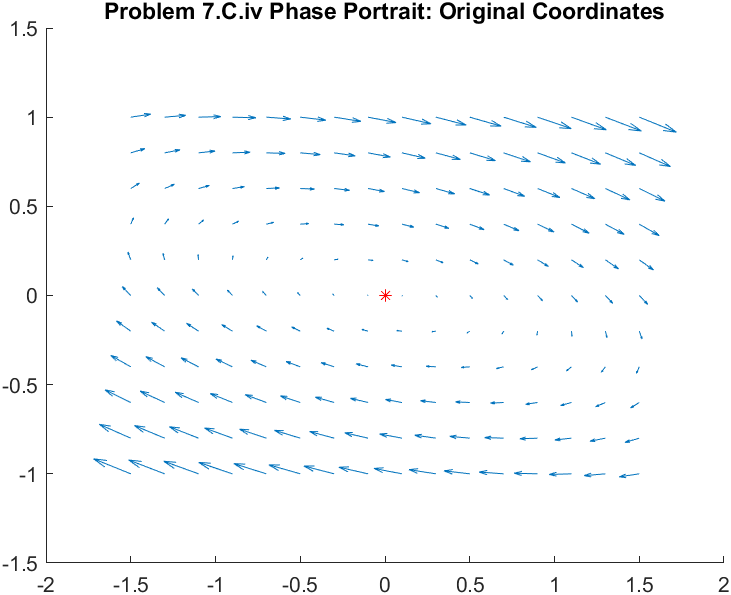
\includegraphics[width=\textwidth,height=.45\textheight,keepaspectratio]{/prob7_img/7_C_iv_Original}
\end{figure}

\begin{figure}[h]
  \centering
  % 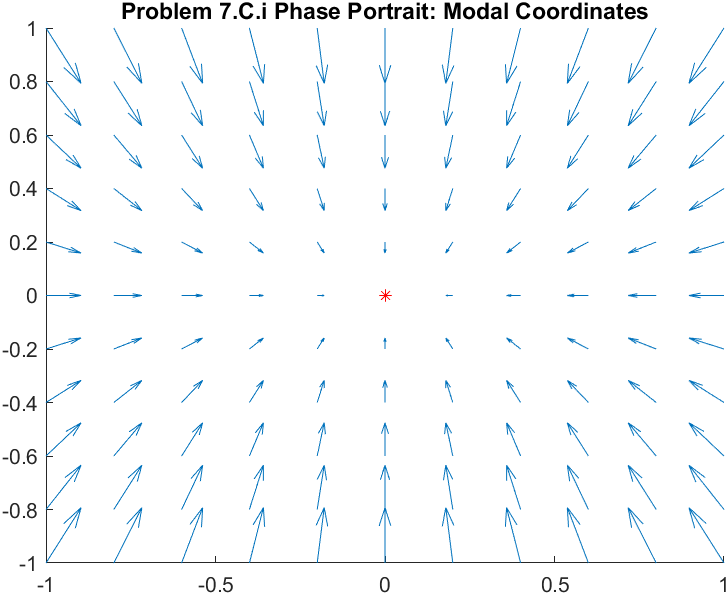
\includegraphics[width=\linewidth]{/prob7_img/7_C_i_modal}
  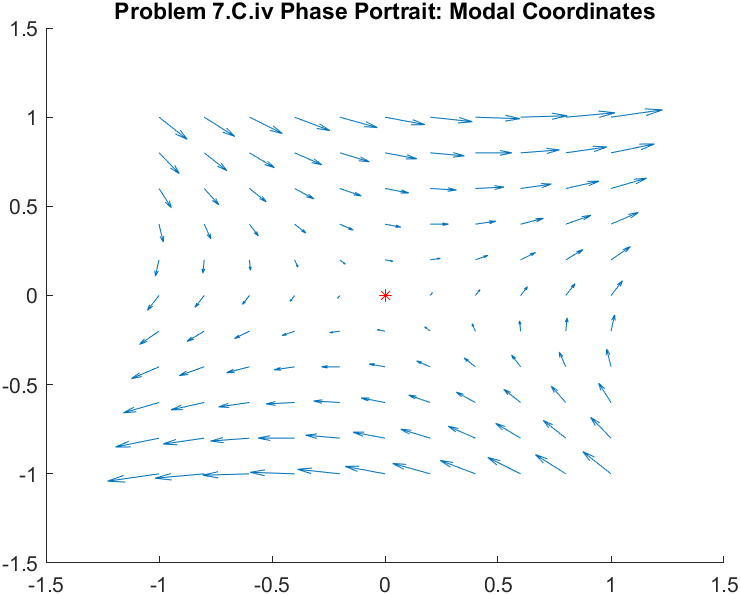
\includegraphics[width=\textwidth,height=.45\textheight,keepaspectratio]{/prob7_img/7_C_iv_modal}

\end{figure}

\begin{figure}[h]
  \centering
  % 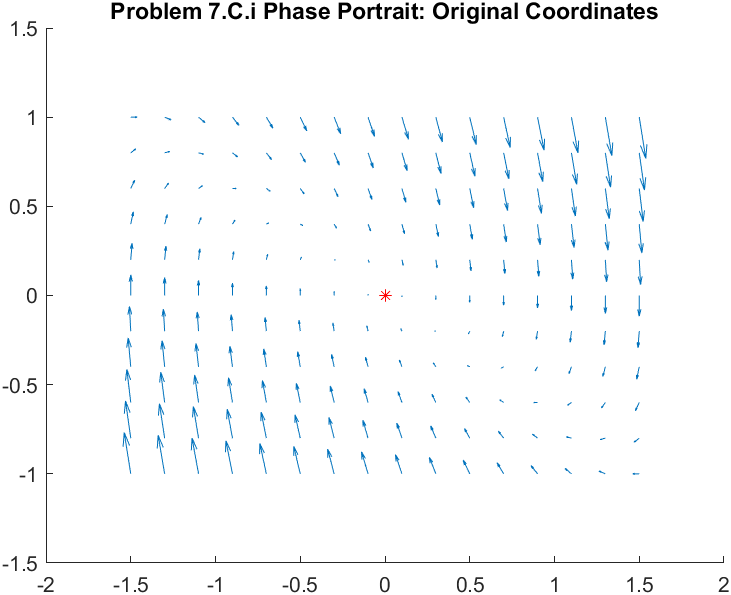
\includegraphics[width=\linewidth]{/prob7_img/7_C_i_Original}
  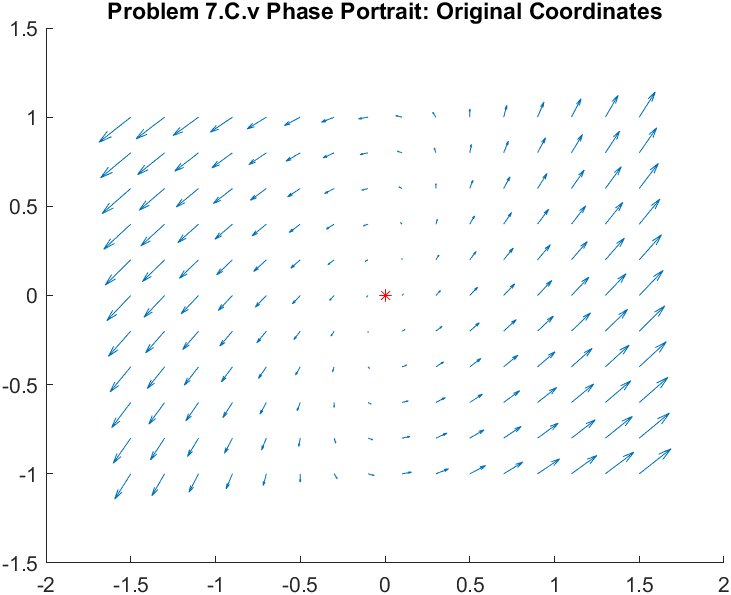
\includegraphics[width=\textwidth,height=.45\textheight,keepaspectratio]{/prob7_img/7_C_v_Original}
\end{figure}

\begin{figure}[h]
  \centering
  % 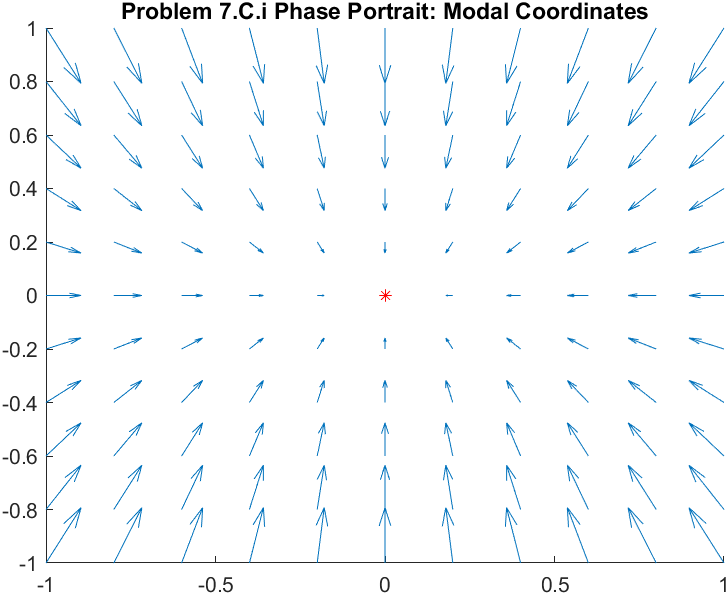
\includegraphics[width=\linewidth]{/prob7_img/7_C_i_modal}
  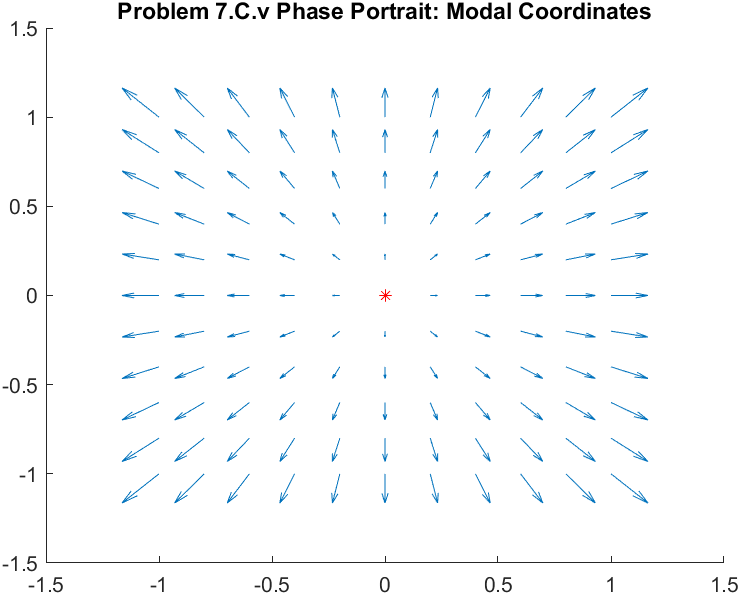
\includegraphics[width=\textwidth,height=.45\textheight,keepaspectratio]{/prob7_img/7_C_v_modal}

\end{figure}

\section*{Problem \#8}


$$
\begin{array}{l}
\dot{x}_{1}=-x_{1}-\frac{x_{2}}{\ln \sqrt{x_{1}^{2}+x_{2}^{2}}} \\
\dot{x}_{2}=-x_{2}+\frac{x_{1}}{\ln \sqrt{x_{1}^{2}+x_{2}^{2}}}
\end{array}
$$


\subsection*{Part A}

After applying Linearization to given system, using a first order Taylor Exspansion, we show that the system produces the following partial derivatives, which will be used to construct the Jacobian matrix for the system.

\begin{flalign*}
  & \frac{\partial f_1}{\partial x_1} = \frac{x_{1} x_{2}}{{\ln\left(\sqrt{{x_{1}}^2+{x_{2}}^2}\right)}^2\left({x_{1}}^2+{x_{2}}^2\right)}-1 \\
  & \frac{\partial f_1}{\partial x_2} = \frac{{x_{2}}^2}{{\ln\left(\sqrt{{x_{1}}^2+{x_{2}}^2}\right)}^2 \left({x_{1}}^2+{x_{2}}^2\right)}-\frac{1}{\ln\left(\sqrt{{x_{1}}^2+{x_{2}}^2}\right)} \\
  & \frac{\partial f_2}{\partial x_1} = \frac{1}{\ln\left(\sqrt{{x_{1}}^2+{x_{2}}^2}\right)}-\frac{{x_{1}}^2}{{\ln\left(\sqrt{{x_{1}}^2+{x_{2}}^2}\right)}^2 \left({x_{1}}^2+{x_{2}}^2\right)} \\
  & \frac{\partial f_2}{\partial x_2} =-\frac{x_{1} x_{2}}{{\ln\left(\sqrt{{x_{1}}^2+{x_{2}}^2}\right)}^2\left({x_{1}}^2+{x_{2}}^2\right)}-1 \\
\end{flalign*}

\noindent After performing these calculations, and eveluating the system at its $x_eq = (0, 0)$, we can constuct the Jacobian matrix $ A_j$ such that the linear system can be written as...

$$
\dot{x} = A_j \cdot x
$$

\noindent Where the Jacobian is defined as...

$$
A_j =
\begin{bmatrix}
  -0.8693 & 0.6419 \\
  -0.6419 & -1.1307
\end{bmatrix}
$$

\noindent By taking the eigenvalues of the linearized systen (described by $A_j$), we can attempt to asses local stability of the system.

$$
\text{eigenvalue} = -1.0000 \pm 0.6285i
$$

\noindent Since the `real' component of the eigenvalue is in the left-half of the complex plane, than we would presume that the system is \underline{stable}; however, since the eigenvalues are complex, this means that the linearized system would indicate that the equilibrium point is a \underline{\textbf{stable focus}}.

\subsection*{Part B}

\subsection*{Part C}

\section*{Problem \#9}

\subsection*{Part 1}

$$
\begin{array}{l}
\dot{x}_{1}=x_{2} \\
\dot{x}_{2}=x_{1}-2 \tan ^{-1}\left(x_{1}+x_{2}\right)
\end{array}
$$

\noindent The behavior of this phase portrait is a bit unusual. While at first glance, it looke like a stable node, at the edges of the plot, we can see that there are diverging vector which might indictate that this system is more complicated than one might think at first glance.


\begin{figure}[h]
  \centering
  % 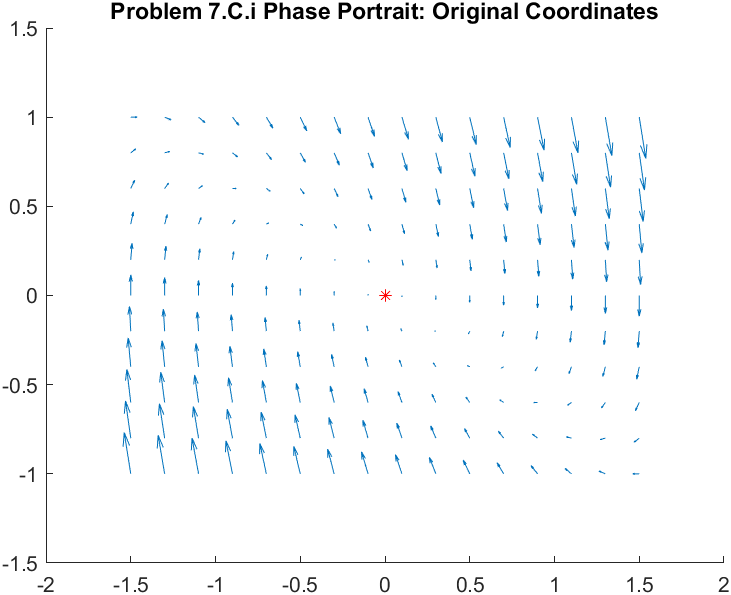
\includegraphics[width=\linewidth]{/prob7_img/7_C_i_Original}
  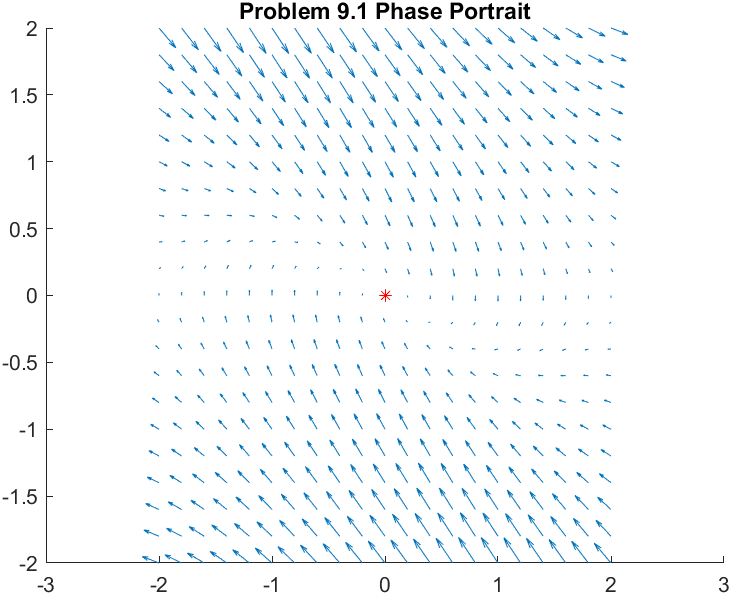
\includegraphics[width=\textwidth,height=.45\textheight,keepaspectratio]{/prob9_img/portrait_9_1}
\end{figure}

\subsection*{Part 2}

$$
\begin{array}{l}
\dot{x}_{1}=x_{2} \\
\dot{x}_{2}=-x_{1}+x_{2}\left(1-3 x_{1}^{2}-2 x_{2}^{2}\right)
\end{array}
$$

\noindent The behavior of this phase portrait is unsual in the fact that the vector field is approaching the $y = 0$ vertically from both the positive and negative directions. This might indictate that the system as a continuum, equilibrium along this line. The other interesting behavior of this system is that it the magnitude of the vector field is more pronouced at the extremes of the plot and quickly dies down in the neighborhood around the origin.

\begin{figure}[h]
  \centering
  % 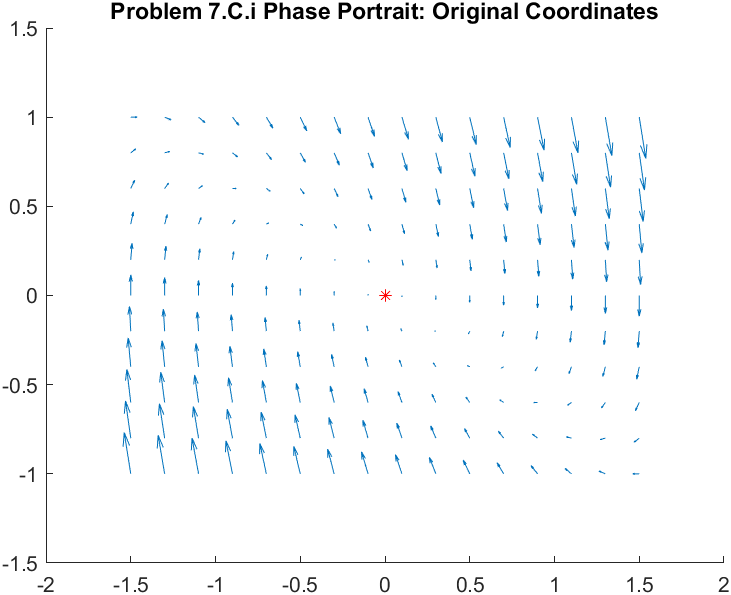
\includegraphics[width=\linewidth]{/prob7_img/7_C_i_Original}
  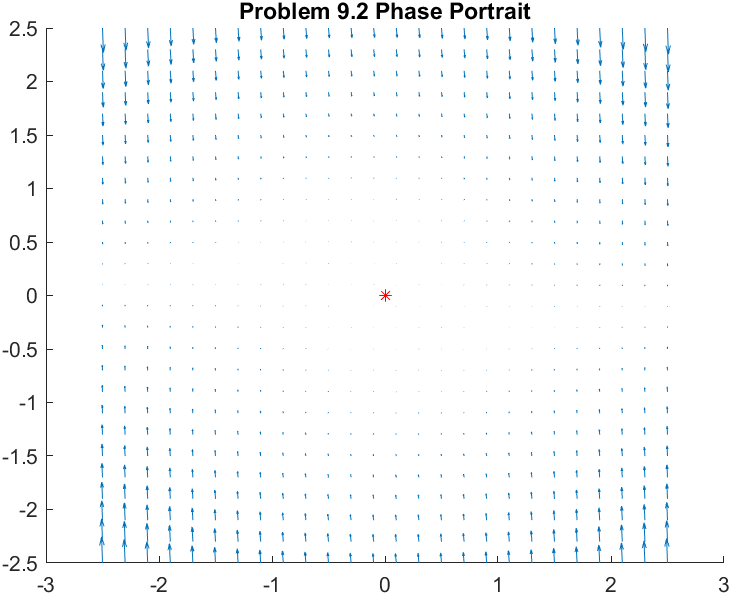
\includegraphics[width=\textwidth,height=.45\textheight,keepaspectratio]{/prob9_img/portrait_9_2}
\end{figure}


\subsection*{Part 3}

$$
\begin{array}{l}
\dot{x}_{1}=x_{1}-x_{1} x_{2} \\
\dot{x}_{2}=2 x_{1}^{2}-x_{2}
\end{array}
$$

\noindent This phase portrait apears to show that the system is strongly unstable about the origin (and the entire domain of the plot), as the vector field has a large magnitude throughout the plot. None of which converge to the origin. However, the most interesting feature of this plot is how regular the features are and how the system propigates to the left in almost perfectly horizontal lines. This means that from any initial condition starting inside the domain of the plane, the phase prortrait doesn't appear to converge, however it merely forces the system to transit to the left. While I cannot say for sure, in theory I could see this being the property of a vertical continuum equilibrium point at some point beyond the scope of the plot. However it is also possible that the system is actually well defined, but requires a must larger domain so that to see the pattern.

\begin{figure}[hb!]
  \centering

  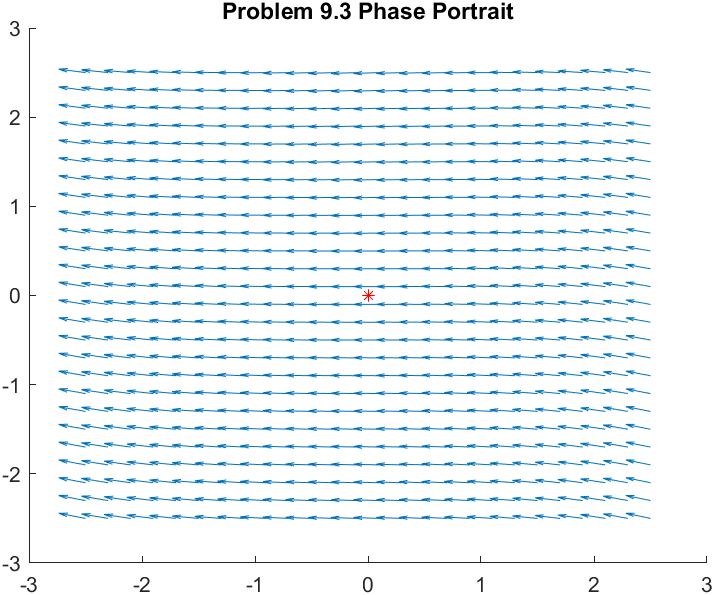
\includegraphics[width=\textwidth,height=.45\textheight,keepaspectratio]{/prob9_img/portrait_9_3}
\end{figure}


\subsection*{Part 4}

$$
\begin{array}{l}
\dot{x}_{1}=x_{1}+x_{2}-x_{1}\left(\left|x_{1}\right|+\left|x_{2}\right|\right) \\
\dot{x}_{2}=-2 x_{1}+x_{2}-x_{2}\left(\left|x_{1}\right|+\left|x_{2}\right|\right)
\end{array}
$$

\noindent Similar to the second phase protrait, we see what appears to be a continuous horizontal line of equilibrium at $y=0$. The vector fields approach that line nearly perfectly vertically from both the top and bottom directions. While this plot is very much like the other plot, the vector field about the line $x = 0$, is must more pronounced.

\begin{figure}[h]
  \centering
  % 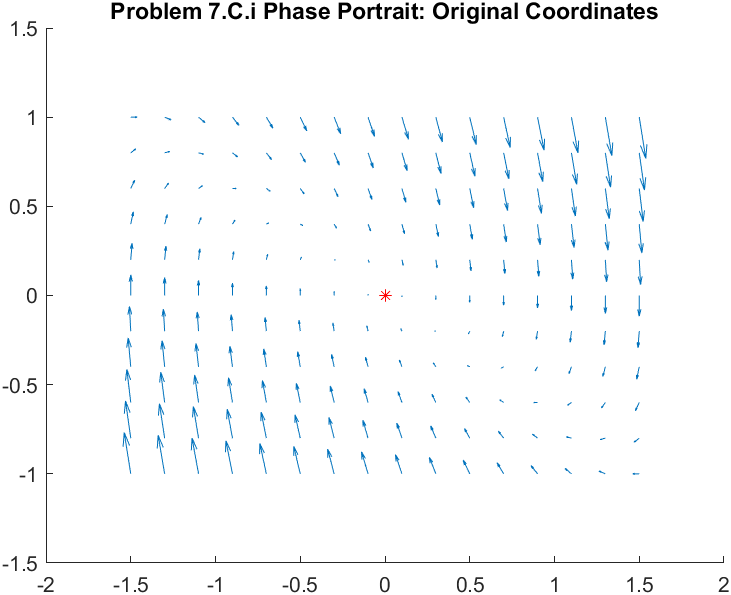
\includegraphics[width=\linewidth]{/prob7_img/7_C_i_Original}
  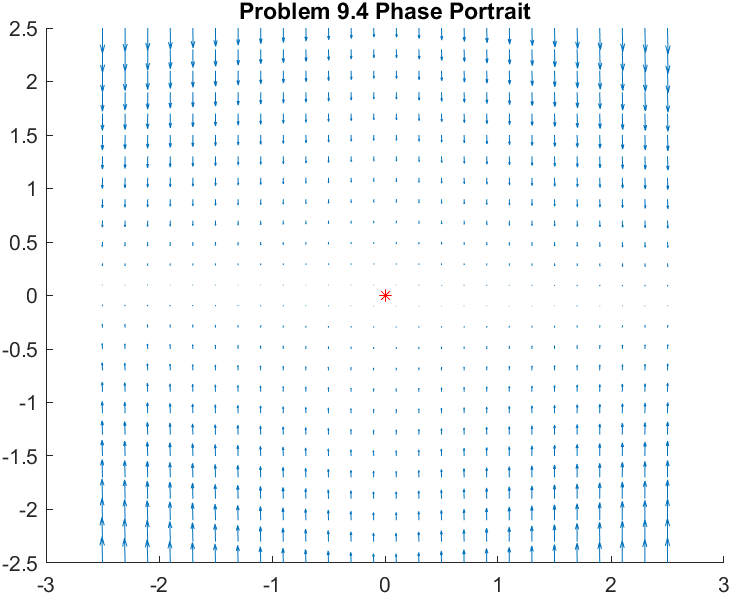
\includegraphics[width=\textwidth,height=.45\textheight,keepaspectratio]{/prob9_img/portrait_9_4}
\end{figure}


\section*{Problem \#10}

Missing information. Problem not required

\section*{Problem \#11}

For $x = \R^{n}$ ...

\noindent Given norm equivalence ...
$$ c\left\Vert x \right\Vert_{a} \leq \left\Vert x \right\Vert_{b} \leq d \left\Vert x \right\Vert_{a} $$

\subsection*{11.1}
For the problem ...

$$ \left\Vert x \right\Vert_{2} \leq \left\Vert x \right\Vert_{1} \leq \sqrt{n} \left\Vert x \right\Vert_{2} $$

\noindent From the statement of the norm equivalence it is clear that there exist norms such that $a=2$ and $b=1$ and that constants $c=1$ and $d=\sqrt{n}$ exist and satisfy the inequality.

\subsection*{11.2}

For the problem ...

$$ \left\Vert x \right\Vert_{\infty} \leq \left\Vert x \right\Vert_{2} \leq \sqrt{n} \left\Vert x \right\Vert_{\infty} $$

\noindent Similar to the previous problem, we can show through norm equivalence that for $a=\infty$ and $b=2$ and that constants $c=1$ and $d=\sqrt{n}$ exist and satisfy the inequality.

\subsection*{11.3}

For the problem ...

$$ \left\Vert x \right\Vert_{\infty} \leq \left\Vert x \right\Vert_{1} \leq \sqrt{n} \left\Vert x \right\Vert_{\infty} $$

\noindent Similar to the previous problem, we can show through norm equivalence that for $a=\infty$ and $b=2$ and that constants $c=1$ and $d=n$ exist and satisfy the inequality.


\section*{Problem \#12}

Given the set $S = \{x \in \R^2 | -1 < x_{i} \leq 1, i = 1,2\}$.

\begin{enumerate}
    \item The set S is not open since it does not contain all of it's limit points. This is due to the lack of equality on the negative bound of $x_i$.
    \item The closure of set S is the set $\bar{S} = S \cup \{ Limit Points \}$. Which is defined as ...\\  $\bar{S} = \{ x\in \R^2 | -1 \leq x_{i} \leq 1, i = 1,2 \}$

    \item $ S_{interior}$ are all of the points contained in the set and not on the boundary. \\

    $S_{interior} = \{ x \in \R^2 | -1 < x_{i} < 1, i = 1,2 \}$

    \item $S_{boudary}$ is defined to be $\bar{S} - S$. Such that... \\
    $S_{boudary} = \{ x\in\R^2 | \: x_{i} = -1 \text{ or } x_{i} =1, i = 1,2 \}$
\end{enumerate}


\section*{Problem \#13}

\[
u_T(t) =
\begin{cases}
    0 & \text{if $t<T $} \\
    1 & \text{if $t\geq T$}
\end{cases}
\]

\subsection*{Part 13.A}

The unit step function $u_T(t)$ is piecewise continuous if it is continuous on each piecewise segment, of the function, withonly a finite number of discontinuities. \\

In order to prove this the limit (defined from both the positive and negative approach) much exist for each value on the function segment. \\

Since the unit step function is piecewise, all that needs to be done is to prove the continuity for both segments of the function, with the exception of the jump discontinuity that is known to exist at $t = T$.

\begin{flalign*}
    & \lim_{t\to t^{+}} u_T(t) = 0 \hspace{2cm}\forall t<T \\
    & \lim_{t\to t^{-}} u_T(t) = 0
\end{flalign*}

\noindent This is true for any point on the first segment of the unit step. This is also valid for the second segment of the unit step as follows.

\begin{flalign*}
    & \lim_{t\to t^{+}} u_T(t) = 1 \hspace{2cm}\forall t\geq T \\
    & \lim_{t\to t^{-}} u_T(t) = 1
\end{flalign*}

\noindent \textbf{Solution:} Since we have shown the unit step function is continuous on each segement, with the known exception of the ``jump discontinuity,'' we can state that this function is piecewise continuous.


\subsection*{Part 13.B}

Show that $f(t) = g(t)u_T(t)$, for any continuous function $g(t)$ is piecewise continuous. \\

Similar to the previous problem, we can demonstrate that $U_T(t)$ is know to be peicewise continuous. Given the fact that $g(t)$ is known to be continuous, we can exploit these two known characteristics to state that the product of these functions must be piecewise continuous. This is due to the fact that piecewise continuity is a weaker condition than the general continuity of a function and therefore the product of continuous and piecewise continuous function must also retain this weaker form of continuity. \\

This can be shown using the existance of the limit of the product of the functions, such that if the limit exists (from both the positive and negative approach) for each segment of the Unit step function, then the product of the unit step function with the continuous function, must also be piecewise continuous. \\

\begin{flalign*}
    & \lim_{t\to t^{+}} g(t) \cdot u_T(t) = 0 \hspace{2cm}\forall t <  T \\
    & \lim_{t\to t^{-}} g(t) \cdot u_T(t) = 0
\end{flalign*}

\begin{flalign*}
    & \lim_{t\to t^{+}} g(t) \cdot u_T(t) = 1 \cdot g(t) \hspace{2cm}\forall t \geq T \\
    & \lim_{t\to t^{-}} g(t) \cdot u_T(t) = 1 \cdot g(t)
\end{flalign*}

\noindent \textbf{Solution:} Since the value of $g(t)$ for any valid $t$ on that peicewise linesegment must be continuous, the product of $1$ times $g(t)$ must be continuous, and since we have already shown that $u_T(t)$ is continuous on its defined interval, the piecewise agregation of these segments into function $f(t)$ must also be piecewise continuous.


\subsection*{Part 13.C}

Since a periodic square waveform is a piecewise assembly of many unit step functions $u_T(t)$ defined for different values of $T$ defined as $T = n \cdot P \: \text{where} \: n= 0, 1,2,3 \cdots$ and where $P$ is the prescribed period of the waveform.  \\

By observation is should be clear that the piecewise assembly of a piecewise continuous functions itself should be piecewise continuous, with the exception of the jump discontinuities of the original step function. This can be shown by repeating the proof for the existance of the limit for each segment of the piecewise assembly of functions; however is skipped for brevity.


\section*{Problem \#14}


\section*{Problem \#15}

\subsubsection*{15.1.A}
For ...

$$
f(x) =
\begin{cases}
    x^{2}sin(1/x), & \text{for $x\neq0 $} \\
    0, & \text{for $x =0$}
\end{cases}
$$

The function is \textbf{not} continuously differentiable since even though the derivative for the function exists there is an essential discontinuity at $x =0$ for the derivative of the function, where the limit does not exist. As such it is not Continuously Differentiable.
\subsubsection*{15.1.B}

The function $f(x)$ \textbf{is} locally Lipschitz at $x=0$, since there exists an `L' which satisfies the Lipschitz inequality, for every possible point $(x_1, x_2) \in B_r  $.

\subsubsection*{15.1.C}

The function $f(x)$ is not strictly speaking `continuous' at $x=0$, since it is a piecewise function, with an obvious discontinuity at $x=0$, however in so much as the domain of continuity is $x=0$, the \textbf{yes} its continuous at that point.

\subsubsection*{15.1.D}

The function $f(x)$ is \textbf{not} globally Lipschitz continuous since there is no `single' constant L which satisfies the Lipschitz inequality for each point $(x,y) \in \R$.

\subsubsection*{15.1.E}

The function $f(x)$ is \textbf{not} `uniformly continuous' on $\R$. It would be uniformly continuous on a bounded interval.

\subsubsection*{15.1.F}

The function $f(x)$ is Lipschitz on the interval $[-1, 1]$, since there exists a `L' over that interval which satisfies the Lipschitz inequality.


\subsection{}

For ...

$$
f(x) =
\begin{cases}
    x^{3}sin(1/x), & \text{for $x\neq0 $} \\
    0, & \text{for $x =0$}
\end{cases}
$$


\subsubsection*{15.2.A}

The function $f$ is differentiable over its entire domain, however, there is discontinuity at $x=0$. However, when the domain of the continuity is restricted to the point $x=0$, the function \textbf{is} continuously differentiable at that point.

\subsubsection*{15.2.B}

The function $f$ is Locally Lipschitz at the point $x=0$.

\subsubsection*{15.2.C}

The function $f$, is not continuous over its entire domain; however, when restricted to the point $x=0$ the function \textbf{is} continuous at that point.

\subsubsection*{15.2.D}
The functino $f$ is \textbf{not} gloablly Lipschitz since its derivative is not boundedin $\R$.
\subsubsection*{15.2.E}

The function $f$ is \textbf{not} uniformly continuous since the there exists a $\delta$ which does not satisfy the condition for uniform continuity given an $\epsilon$.
\subsubsection*{15.2.F}

The function $f$ \textbf{is} Lipschitz on the bounded interval $[-1 , 1]$ since there exists an L which can bound the function according to its definition.


\subsection{}

For ...

$$
f(x) = tan\left( \frac{\pi x}{2}\right)
$$

\subsubsection*{15.3.A}
The functino $f$ \textbf{is} continuously differentiable at $x=0$, since both the function and derivative of $f$ exist when taken in the limit at $x=0$.

\subsubsection*{15.3.B}

Given $y =.25$ and $x=0$

$$
\left\Vert f(y) - f(x) \right\Vert \leq L \left\Vert y -x \right\Vert
$$

$$
\left\Vert .25534 - 0 \right\Vert \leq L \left\Vert .25 - 0 \right\Vert
$$

Where if $L =2$, the Lipschitz condition \textbf{is} satisfied in ball centered around the point $x=0$.

\subsubsection*{15.3.C}

Using the Limit evaluation of a function, it can be shown the that the function $f$ approaches $0$ in the limit. Therefore the function $f$ is continuous at $x=0$.

\subsubsection*{15.3.D}

The function $f$ is \textbf{not} globally Lipschitz, since its derivative is not bounded.

\subsubsection*{15.3.E}

The function $f$ is not uniformly continuous since, due to nature of the tanget function, the verticle asymptotes prevent there existing a single $\delta$ that satisfies the condition for uniform continuity given a single $\epsilon$.


\subsubsection*{15.3.F}
The functino $f$ \textbf{is} Lipschitz on the interval $[-1, 1]$.








\section*{Problem \#16}

\subsubsection*{16.1.A}

The function $f$ is \textbf{not} continuously differentiable due to the discontinuities in the sign function.
\subsubsection*{16.1.B}

The function $f$ \textbf{is} locally Lipschitz, which can be demonstrated by evaluation.
\subsubsection*{16.1.C}

The function $f$ is \textbf{not} continuous on $\R^n$, due to the discontinuity at $x =0$.
\subsubsection*{16.1.D}

The function $f$ \textbf{is} globally Lipschitz, since the derivative of the function is bounded in $\R^n$.
\subsubsection*{16.1.E}

Since the function is globally Lipschitz, the function must also be Uniformly Continuous.

\subsubsection*{16.2.A}

The function $f$ \textbf{is not} continuously differentiable due to the inclusion of the saturation function.

\subsubsection*{16.2.B}

The function $f$ \textbf{is} locally Lipschitz continuous, for a ball $B_r$.

\subsubsection*{16.2.C}

The function $f$ \textbf{is} continuous on $\R^n$ since there are no discontinuities, for the linear, sine, and saturation functions.

\subsubsection*{16.2.D}

The function $f$ is \textbf{is} globally Lipschitz due to the derivative of the linear, sine, and saturation functions being bounded in $\R^n$.

\subsubsection*{16.2.E}
Since the function is globally Lipschitz, it follows that it \textbf{must} be uniformly continuous over $\R^n$.


\subsubsection*{16.3.A}

The function $f$ \textbf{is not} continuously differentiable, due to the saturation function containing non differentiable sharp points.

\subsubsection*{16.3.B}

The function $f$ \textbf{is} locally Lipschitz, since we can find a ball which is a subset of the $\R^n$ such that the Lipschitz condition holds.
\subsubsection*{16.3.C}

The function $f$ is continuous over $\R^n$.
\subsubsection*{16.3.D}

The function $f$ \textbf{is not} globally Lipschitz since, its derivative is not bounded on $\R^n$
\subsubsection*{16.3.E}

The function $f$ is \textbf{not} uniformly continuous, since for a single $\epsilon$ we cannot find a single $\delta$, which satisfy the continuity condition. Hence the function cannot be uniformly continuous.


\section*{Problem \#17}

Given the P-Norm...

$$
\left\Vert x\right\Vert_{p} \triangleq \left( \sum_{i = 1}^{n} |x_{i}| \right)^{\frac{1}{p}}
$$

\noindent we can show that for the norm defined at $p = \beta$.

$$
\left\Vert f(y) - f(x) \right\Vert_{\beta} \leq L \left\Vert y - x \right\Vert_{\beta}
$$

\noindent Can be shown via `norm equivalence' to equal...

$$
\cancel{C} \cdot \left\Vert f(y) - f(x) \right\Vert_{\alpha} \leq L \left\Vert y - x \right\Vert_{\alpha} \cdot \cancel{C}
$$

\noindent The `Lipschitz Condition' using $ \left\Vert \cdot \right\Vert_{\alpha}$ is only different from the `Lipschitz Condition' using $\left\Vert \cdot \right\Vert_{\beta}$ by a a constant $C \in \R^{+}$. Therefore since the constant in question cancel out, the norms of both $ \alpha$ \& $\beta$ are equivalent.

\section*{Problem \#18}

\section*{Problem \#19}

\section*{Problem \#20}
A function of $f$ is \textbf{uniformly continuous} if $\forall \: \epsilon > 0 \: \text{ then } \exists \: \delta > 0 \text{ such that }$

$$ \left\Vert f(y) - f(x) \right\Vert < \epsilon \hspace{1cm} \text{ whenever} $$
$$ \left\Vert y - x \right\Vert < \delta $$

\noindent Furthermore, a function $f$ is \textbf{Lipschitz Continuous} if $\exists \: L < \infty$ such that...

$$
\left\Vert f(y) - f(x) \right\Vert \leq L \left\Vert y -x \right\Vert
$$

\noindent We can combine the two statements be defining...

$$ \delta = \frac{\epsilon}{L} $$

\noindent By rewriting the condition for Lipschitz Continuity, and including the expression above, we can show that the `uniform continuity' of a function is `essentially' a form of the Lipschitz condition.

$$ \left\Vert y - x \right\Vert < \delta \Rightarrow \left\Vert f(y) - f(x) \right\Vert \leq L \left\Vert y - x \right\Vert < \epsilon   $$


\noindent Therefore, while being \underline{uniformly continuous} does \textbf{not} imply that a function is Lipschitz Continuous, the fact that Lipschitz Continuous is a stronger assumption on the continuity of a function, any Lipschitz function implies that that function is uniformly continuous. 


\section*{Problem \#21}

This problem is very similar to the formulation of Lyapunov Stability Theorem, with the exception that the bound of the derivative norm is not negative semidefinite, but that it is bounded by the time dependent function $g(t)$.


\noindent If we given with the the system defined so that the  derivative $\dot{x}$ is negative semidefinite, we can show that the solution $x$ is  

\section*{Problem \#22}


Given...

\begin{equation*}
    \begin{aligned}
        & \frac{C_{A}}{dt} = -r_{1} \\
        & \frac{C_{B}}{dt} = r_{1} - r_{2} \\
        & \frac{C_{C}}{dt} = r_{2}
    \end{aligned}
    \qquad \qquad
    \begin{aligned}
        & r_{1} = K_{1}C_{A} \\
        & r_{2} = K_{2}C_{B} \\
    \end{aligned}
\end{equation*}

We can define the states of system to be the concentrations of each species, in the reaction as follows...

\begin{equation*}
    \begin{aligned}
        & x_{1} = C_{A} \\
        & x_{2} = C_{B} \\
        & x_{3} = C_{C} \\
    \end{aligned}
\end{equation*}

From whose definitions we can construct a state space by taking first order time derivatives of each state, and substituting the appropriate expression from the equations given above. \\
$$
\begin{bmatrix}
    \dot{x_{1}} \\
    \dot{x_{2}} \\
    \dot{x_{3}}
\end{bmatrix}
=
\begin{bmatrix}
    -K_{1} & 0 & 0 \\
    K_{1} & -K_{2} & 0 \\
    0 & K_{2} & 0
\end{bmatrix}
\begin{bmatrix}
    x_{1} \\
    x_{2} \\
    x_{3} \\
\end{bmatrix}
$$

Such that a matrix $A$ is define to be...

$$
A =
\begin{bmatrix}
    -K_{1} & 0 & 0 \\
    K_{1} & -K_{2} & 0 \\
    0 & K_{2} & 0
\end{bmatrix}
$$

\subsection*{22.A}
Since we can the constitutive equations for the system are a linear function of its arguments, this problem is \textbf{linear system}, and consequently can be written in matrix form as shown above.

\subsection*{22.B}

Since the system is linear, it can be written via the matrix equation shown below...


    $$    \dot{x} = Ax + Bu \\$$
    $$    y = Cx + Du \\$$

\noindent Where the matrices $A$ and $B$, descripe the state and input dynamics of the system, while matrices $C$ and $D$ describe the outputs of the system.

\begin{equation*}
    \begin{aligned}
        & A =
        \begin{bmatrix}
            -K_{1} & 0 & 0 \\
            K_{1} & -K_{2} & 0 \\
            0 & K_{2} & 0 \\
        \end{bmatrix}
        & B =
        \begin{bmatrix}
            0 \\
            0 \\
            0
        \end{bmatrix}
    \end{aligned}
    \qquad \qquad
    \begin{aligned}
        & C =
        \begin{bmatrix}
            1 & 0 & 0
        \end{bmatrix}
        & D =
        \begin{bmatrix}
            0 \\
        \end{bmatrix}
    \end{aligned}
\end{equation*}


\subsection*{22.C}

The dynamics of the response due to its ``initial conditions'' is shown below for all three states of the system, even though the output of the system can only measure the $X_1$. \\


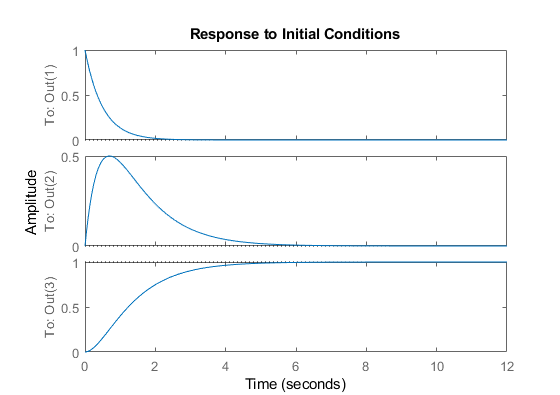
\includegraphics{ss_sim}


\end{document}
